\documentclass[12pt,reqno]{amsart}
\usepackage[top=2cm, left=2cm,right=2cm,bottom=2cm]{geometry}
\renewcommand{\baselinestretch}{1.2}
\usepackage{amsmath}
\usepackage{amssymb}
\usepackage{scalefnt}
\usepackage{tikz}
\usepackage{color,hyperref,enumerate,multicol}
\definecolor{darkblue}{rgb}{0.0,0.0,0.3}
\hypersetup{colorlinks,breaklinks,
            linkcolor=darkblue,urlcolor=darkblue,
            anchorcolor=darkblue,citecolor=darkblue}
            
\usepackage{algorithm}
\usepackage{algorithmic}
\pagestyle{empty}
\newcommand{\N}{\ensuremath{\mathbb{N}}}
\newcommand{\Z}{\ensuremath{\mathbb{Z}}}
\newcommand{\R}{\ensuremath{\mathbb{R}}}
\newcommand{\bL}{\ensuremath{\mathbf{L}}}
\newcommand{\bP}{\ensuremath{\mathbf{P}}}
\newcommand{\bQ}{\ensuremath{\mathbf{Q}}}
\newcommand{\bA}{\ensuremath{\mathbf{A}}}
\newcommand{\bB}{\ensuremath{\mathbf{B}}}
\newcommand{\bG}{\ensuremath{\mathbf{G}}}
\newcommand{\bH}{\ensuremath{\mathbf{H}}}
\newcommand{\invG}{\ensuremath{\operatorname{inv}^{\bG}}}
\newcommand{\invH}{\ensuremath{\operatorname{inv}^{\bH}}}
\newcommand{\meet}{\ensuremath{\wedge}}
\newcommand{\Meet}{\ensuremath{\bigwedge}}
\newcommand{\<}{\ensuremath{\langle}}
\renewcommand{\>}{\ensuremath{\rangle}}
\newcommand{\join}{\ensuremath{\vee}}
\renewcommand{\emptyset}{\ensuremath{\varnothing}}
\renewcommand{\subset}{\ensuremath{\subsetneq}}
\newcommand{\boldemph}{\emph}
\newcommand{\lcm}{\ensuremath{\operatorname{lcm}}}
\newcommand{\Sym}{\ensuremath{\operatorname{Sym}}}
%\newcommand{\bG}{\ensuremath{\mathbf{G}}}

\newcommand{\probskip}{\vskip1cm}

\begin{document}
\thispagestyle{empty}

\noindent \textbf{Math 301} \hskip5cm {\bf Homework 13} \hfill {\bf Fall 2014}
\vskip1cm
\noindent {\bf Exercises:} Chapter 14: 1 (except the $GL_2( {\mathbb R} )$
example), 2, 3, 9, 11 (justify!).\\
{\bf Due date:} Friday, 12/12

\medskip
Recall, if $G$ acts on a set $X$ and $x, y \in X$, then $x$ is said
to be \boldemph{$G$-equivalent} to $y$ if there exists a $g \in G$ such that 
$gx =y$. We  write $x \sim_G y$ or $x \sim y$ if $x$ and $y$ are $G$-equivalent. 
In class, we proved that the $G$-equivalence relation is reflexive and
symmetric. You should check the transitive property on your own to complete the
proof that $\sim$ is an equivalence relation on $X$. 
 
%% \noindent {\bf Exercises:}
\begin{enumerate}
%% 1 %%%%%%%%%%%%%%%%%%%%%%%%%%%%%%%%%%%%%%%%%%%%%%%%
\item[{\bf 14.1}] Each of the examples below describes an action of a group $G$
  on a set $X$, which will give rise to the equivalence relation defined by
  $G$-equivalence.  For each example, compute the equivalence classes of the
  $G$-equivalence relation.  
 
%% {\bf Examples:}
\begin{enumerate}
\item
%\begin{example}{D4_action}
Let $G = D_4$ be the symmetry group of a square.  If $X = \{ 1, 2, 3, 4 \}$ is the set of vertices of the square, then we can consider $D_4$
to consist of the following permutations: 
\[
\{ (1), (13), (24), (1432), (1234), (12)(34), (14)(23), (13)(24) \}.
\]
The elements of $D_4$ act on $X$ as functions.  The permutation $(13)(24)$ acts on vertex 1 by sending it to vertex 3, on vertex 2 by
sending it to vertex 4, and so on.
\mbox{\hspace{1in}}
%% \end{example}

%% In general, if $X$ is any set and $G$ is a subgroup of $S_X$, the
%% group of all permutations acting on $X$, then $X$ is a $G$-set under
%% the group action 
%% \[
%% (\sigma, x) \mapsto \sigma(x)
%% \]
%% for $\sigma \in G$ and $x \in X$.
 
\item 
%% \begin{example}{left_action}
If we let $X = G$, then every group $G$ acts on itself by the so called 
\emph{left regular representation} $\lambda: G \rightarrow \Sym(G)$ which, for
each $g\in G$, gives the function $\lambda_g: G\rightarrow G$ 
defined by $\lambda_g(x) = gx$. That is, $G$
itself is a $G$-set under this ``left multiplication'' action.
%% \begin{gather*}
%% e \cdot x = \lambda_e x = ex = x \\
%% (gh) \cdot x = \lambda_{gh}x = \lambda_g \lambda_h x =
%% \lambda_g(hx) = g \cdot ( h \cdot x).
%% \end{gather*}
Alternatively, we could restrict the domain of $\lambda$ to a particular
subgroup, say, $H\leq G$, and then $G$ becomes an $H$-set under left 
multiplication by elements of $H$. 
%% \end{example}
 
 
\item
%% \begin{example}{conj_action}
Let $G$ be a group and suppose that $X=G$. If $H$ is a subgroup of
$G$, then $G$ is an $H$-set under 
the \emph{conjugation action}; that is, we can define an action 
$\varphi$ of $H$ on $G$ with the function 
$\varphi: H \rightarrow (G \rightarrow G)$ where 
$\varphi_h(g) = hgh^{-1}$.
%% Alternatively, viewing the action as a function of two variables, we have
%% \[
%% \varphi: H \times G \rightarrow G
%% \quad \text{ via } \quad
%% \varphi(h,g)= hgh^{-1}
%% \]
%% for $h \in H$ and $g \in G$.%%   Clearly, the first axiom for a group
%% action holds.  Observing that 
%% \begin{align*}
%% (h_1 h_2, g) 
%% & = h_1 h_2 g (h_1 h_2 )^{-1} \\
%% & = h_1( h_2 g h_2^{-1}) h_1^{-1} \\
%% & =  (h_1, (h_2, g) ),
%% \end{align*}
%% we see that the second condition is also satisfied.
%% %% \end{example}
 
 
\item
%% \begin{example}{left_coset_action}
Let $H$ be a subgroup of $G$ and let $G/H$ denote the set of left cosets
of $H$.  The set $G/H$ is a $G$-set under the action
$\lambda: G \rightarrow (G/H \rightarrow G/H)$ given by 
$\lambda_g(xH) = gxH$.%%   That is,
%% $\lambda: G \times G/H \mapsto G/H$ given by 
%% $\lambda(g, xH) = gxH$.
%% \]
%% That is, for each $g$, for each $xH \in G/H$, we have $\lambda_g(xH) = gxH.$
%% Again, it is easy to see that the first axiom is true. Since $(g g')xH
%% = g( g'x H)$, the second axiom is  also true.
%% \end{example}
 
\end{enumerate}

\item[{\bf 14.2}] \label{actions}
Compute all $X_g$ and all $G_x$ for each of the following permutation
groups. 
\begin{enumerate}
 
 \item
$X= \{1, 2, 3\}$, \\
$G=S_3=\{(1), (12), (13), (23), (123), (132)  \}$
 
 \item
$X = \{1, 2, 3, 4, 5, 6\}$, \\
$G = \{(1), (12), (345), (354), (12)(345), (12)(354)  \}$
 
\end{enumerate}
 
 
\item[{\bf 14.3}]
Compute the $G$-equivalence classes of $X$ for each of the $G$-sets in
Exercise~14.2. For each $x \in X$ verify that 
$|G|=|{\mathcal O}_x| \cdot |G_x|$.  

\item[{\bf 14.9}]
How many ways can the vertices of an equilateral triangle be colored
using three different colors? 

\item[{\bf 14.11}]
Up to a rotation, how many ways can the faces of a cube be colored
with three different colors?  (Justify any formula you use.)
 
\end{enumerate}
\end{document}
%***************Calculations************************

 
\item \label{actions:computation:exercise}
Compute all $X_g$ and all $G_x$ for each of the following permutation
groups. 
\begin{enumerate}
 
 \item
$X= \{1, 2, 3\}$, \\
$G=S_3=\{(1), (12), (13), (23), (123), (132)  \}$
 
 \item
$X = \{1, 2, 3, 4, 5, 6\}$, \\
$G = \{(1), (12), (345), (354), (12)(345), (12)(354)  \}$
 
\end{enumerate}
 
 
\item
Compute the $G$-equivalence classes of $X$ for each of the $G$-sets in
Exercise~\ref{actions:computation:exercise}. For each $x \in X$ verify that $|G|=|{\mathcal O}_x| \cdot
|G_x|$.  
 
 
\item
Let $G$ be the additive group of real numbers. Let the action of
$\theta \in G$ on the real plane ${\mathbb R}^2$ be given by rotating the
plane counterclockwise about the origin through $\theta$ radians. Let
$P$ be a point on the plane other than the origin.
\begin{enumerate}
 
 \item
Show that ${\mathbb R}^2$ is a $G$-set.
 
 \item
Describe geometrically the orbit containing $P$.
 
 \item
Find the group $G_P$.
 
\end{enumerate}
 
 
\item
Let $G =  A_4$ and suppose that $G$ acts on itself by conjugation;
that is, $(g,h)~\mapsto~ghg^{-1}$. 
\begin{enumerate}
 
 \item
Determine the conjugacy classes (orbits) of each element of $G$.
 
 \item
Determine all of the isotropy subgroups for each element of $G$.
 
\end{enumerate}
 
 
\item
Find the conjugacy classes and the class equation for each of the
following groups. 
\begin{multicols}{4}
\begin{enumerate}

\item
$S_4$

\item
$D_5$

\item
${\mathbb Z}_9$

\item
$Q_8$


\end{enumerate}
\end{multicols}
 

 
 
\item  %%%%%%%%%%%%%%%%
Write the class equation for $S_5$ and for $A_5$.
 
 
\item
If a square remains fixed in the plane, how many different ways can
the corners of the square be colored if three colors are used?
 
 
\item
How many ways can the vertices of an equilateral triangle be colored
using three different colors? 
 
 
\item
Find the number of ways a six-sided die can be constructed if each
side is  marked differently with $1, \ldots, 6$ 
dots.
 
\item
Up to a rotation, how many ways can the faces of a cube be colored
with three different colors? 
 
 
 
\item
Consider 12 straight wires of equal lengths with their ends soldered
together to form the edges of a cube. Either silver or copper wire can be
used for each edge.  How many different ways can the cube be
constructed? 
 
 
 
\item
Suppose that we color each of the eight corners of a cube. Using three
different colors, how many ways can the corners be colored up to a
rotation of the cube? 
 
 
\item
Each of the faces of a regular tetrahedron can be painted either red
or white.  Up to a rotation, how many different ways can the
tetrahedron be painted? 
 
 
\item
Suppose that the vertices of a regular hexagon are to be colored either
red or white.  How many ways can this be done up to a symmetry  of the
hexagon? 
 
 
\item
A molecule of benzene is made up of six carbon atoms and six hydrogen
atoms, linked together in a hexagonal shape as in Figure~\ref{benzene}.
\begin{enumerate}
 
 \item
How many different compounds can be formed by replacing one or more of
the hydrogen atoms with a chlorine atom? 
 
 \item
Find the number of different chemical compounds that can be formed by
replacing three of the six hydrogen atoms in a benzene ring with a
$CH_3$ radical.
 
\end{enumerate}
 
 
\begin{figure}[ht]
\begin{center}
\tikzpreface{actions_benzene}
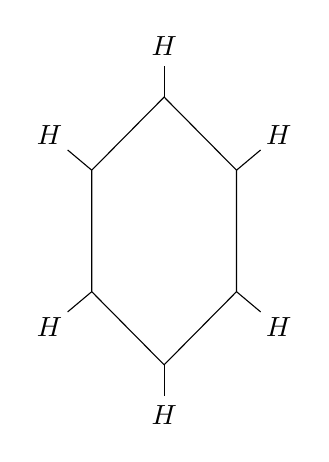
\begin{tikzpicture}[scale=1.0] %%Replaced figure with tikz figure - TWJ 6/28/2010

\draw (40:1.2) -- (90:1.7) -- (140:1.2) -- (220:1.2) -- (270:1.7) -- (320:1.2) -- cycle;
\draw (90:1.7) -- (90:2.1) node [above] {$H$};
\draw (270:1.7) -- (270:2.1) node [below] {$H$};
\draw (40:1.2) -- (40:1.6);
\node at (40:1.9) {$H$};
\draw (140:1.2) -- (140:1.6);
\node at (140:1.9) {$H$};
\draw (220:1.2) -- (220:1.6);
\node at (220:1.9) {$H$};
\draw (320:1.2) -- (320:1.6);
\node at (320:1.9) {$H$};

\end{tikzpicture}
\end{center}
\caption{A benzene ring}
\label{benzene}
\end{figure}
 
 
\item
How many equivalence classes of switching functions are there if the
input variables $x_1$, $x_2$, and $x_3$ can be permuted by any
permutation in $S_3$? What if the input variables $x_1$, $x_2$, $x_3$,
and $x_4$ can be permuted by any permutation in $S_4$?
 
 
\item
How many equivalence classes of switching functions are there if the
input variables $x_1$, $x_2$, $x_3$, and $x_4$ can be permuted by any
permutation in the subgroup of $S_4$ generated by the permutation
$(x_1 x_2 x_3 x_4)$?  
 
 
\item
A striped necktie has 12 bands of color. Each band can be colored
by one of four possible colors.  How many possible different-colored
neckties are there? 
 
 
%***************Theory******************************
 
 
\item
A group acts \boldemph{faithfully} on a $G$-set $X$ if the identity is the
only element of $G$ that leaves every element of $X$ fixed. Show that
$G$ acts faithfully  on $X$ if and only if no two distinct elements of
$G$ have the same action on each element of $X$.
 
 
\item
Let $p$ be prime. Show that the number of different abelian groups of
order $p^n$ (up to isomorphism)  is the same as the number of
conjugacy classes in $S_n$. 
 
 
\item
Let $a \in G$. Show that for any $g \in G$, $gC(a) g^{-1} =
C(gag^{-1})$. 
 
 
\item
Let $|G| = p^n$ and suppose that $|Z(G)| = p^{n-1}$ for  $p$ prime.
Prove that $G$ is abelian. 
 
 
\item
Let $G$ be a group with order $p^n$ where $p$ is prime and $X$ a
finite $G$-set.  If $X_G = \{ x \in X : gx = x \text{ for all }g \in
G \}$ is the set of elements in $X$ fixed by the group action, then
prove that $|X| \equiv |X_G| \pmod{ p}$.

\item
If $G$ is a group of order $p^n$, where $p$ is prime and $n \geq 2$, show that $G$ must have a proper subgroup of order $p$.  If $n \geq 3$, is it true that $G$ will have a proper subgroup of order $p^2$?
%Moved problem from cosets.tex TWJ 12/19/2011
 
 
\end{enumerate}
}
 
 
 
\subsection*{Programming Exercise}
 
 
 
{\small
Write a program to compute the number of conjugacy classes in $S_n$.
What is the largest $n$ for which your program will work?
}
 
 
 
\subsection*{References and Suggested Reading} %%TWJ 6/28/2010 - References checked.
 
 
 
{\small
\begin{itemize}
 
\item[\textbf{[1]}]
De Bruijin, N. G. ``P\'{o}lya's Theory of Counting,'' in {\it
Applied Combinatorial Mathematics}, Beckenbach, E. F., ed.
Wiley, New York, 1964.
 
\item[\textbf{[2]}]
Eidswick, J. A. ``Cubelike Puzzles---What Are They and How
Do You Solve Them?'' \textit{American Mathematical
Monthly} \textbf{93} (1986), 157--76.
 
\item[\textbf{[3]}]
Harary, F., Palmer, E. M., and Robinson, R. W. ``P\'{o}lya's
Contributions to Chemical Enumeration,'' in \textit{Chemical
Applications of Graph Theory}, Balaban, A. T., ed. Academic
Press, London, 1976.
 
\item[\textbf{[4]}] %%TWJ 6/28/2010 - This is out of print
G{\aa}ding, L. and Tambour, T. \textit{Algebra for Computer
Science}. Springer-Verlag, New York, 1988.
 
\item[\textbf{[5]}] %%TWJ 6/28/2010 - This is out of print
Laufer, H. B. \textit{Discrete Mathematics and Applied Modern
Algebra}. PWS-Kent, Boston, 1984.
 
 
\item[\textbf{[6]}] %%TWJ 6/28/2010 - This is out of print
P\'{o}lya, G. and Read, R. C. \textit{Combinatorial Enumeration
of Groups, Graphs, and Chemical Compounds}. Springer-Verlag,
New York, 1985.
 
\item[\textbf{[7]}]
Shapiro, L. W. ``Finite Groups Acting on Sets with
Applications,'' \textit{Mathematics Magazine}, May--June 1973,
136--47.
 
\end{itemize}
}
 
\sagesection
 



